\section{BCE model}
I dette, har vi opfyldt kravet omkring en BCE model til at dokumentere og skabe oveblik over vores kendskab i koden.


Vi har igen brugt \texttt{Game} som vores \textit{Controller}, der uddeler ansvaret til de andre klasser. Ud over det er det de samme \textit{Entities} og \textit{Boundaries}, som i \cite{19del2}.

I forhold til en optimal \textbf{BCE model}, har måttet ændre lidt i dens kendskaber. Efter at have sammenlignet koden med vores udgangspunkt, har vi måttet lave kendskab begge veje mellem \texttt{Gameboard} og \texttt{Field}. Samtidig fik vi et krav i opgaven, at \texttt{Field} skulle kunne kalde objekter af \texttt{Player}. Derfor har vi også måttet lave et kendskab der.

Kendskabet til \texttt{DieCup} har vi flyttet over i \texttt{GameBoard}, for at få det til at passe med vores nye \textbf{Domæne Model}, og for at sørge for \texttt{Game} ikke blev bloated af ansvarsopgaver.

Overblikket over dette kan ses i figur \vref{fig:bcemodel}

\begin{figure}[ht]
\centering
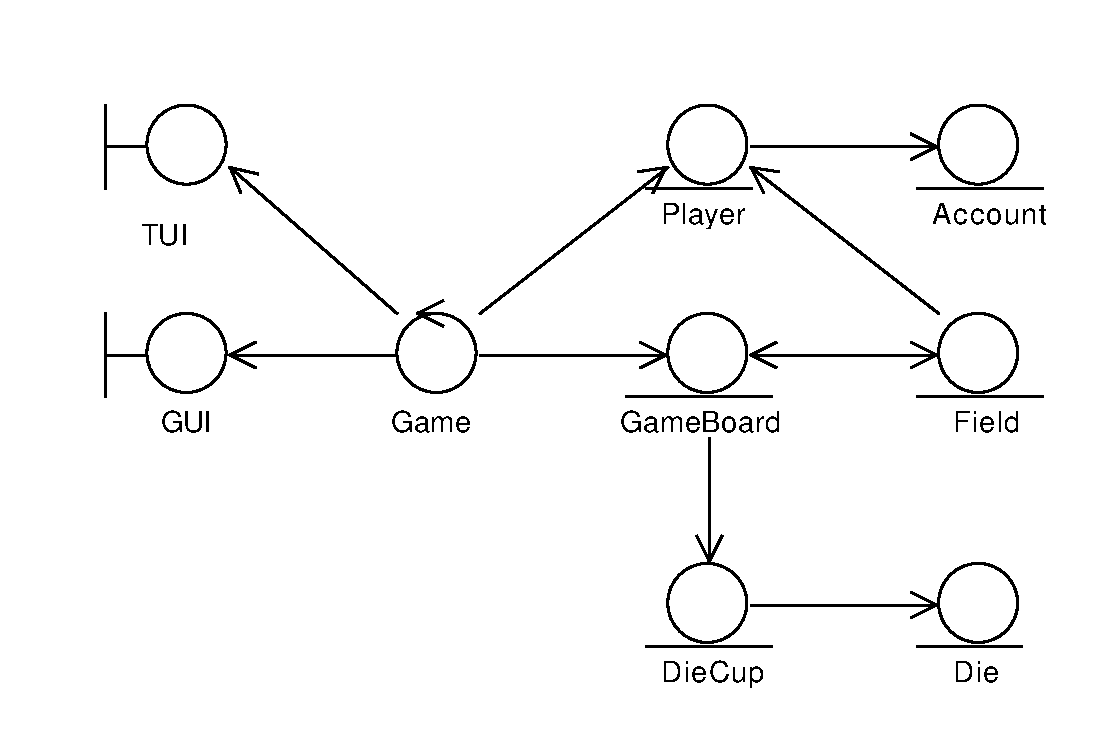
\includegraphics[width=1\textwidth]{BCEModel.pdf}
\caption[<Text for the list of figures>]{BCE Model}
\label{fig:bcemodel}
\end{figure}
\newpage